\section{Particle accelerators and colliders}
This is a very quick overview of the most important types of particle
physics accelerators/colliders.

\begin{figure}[!h]
\centering
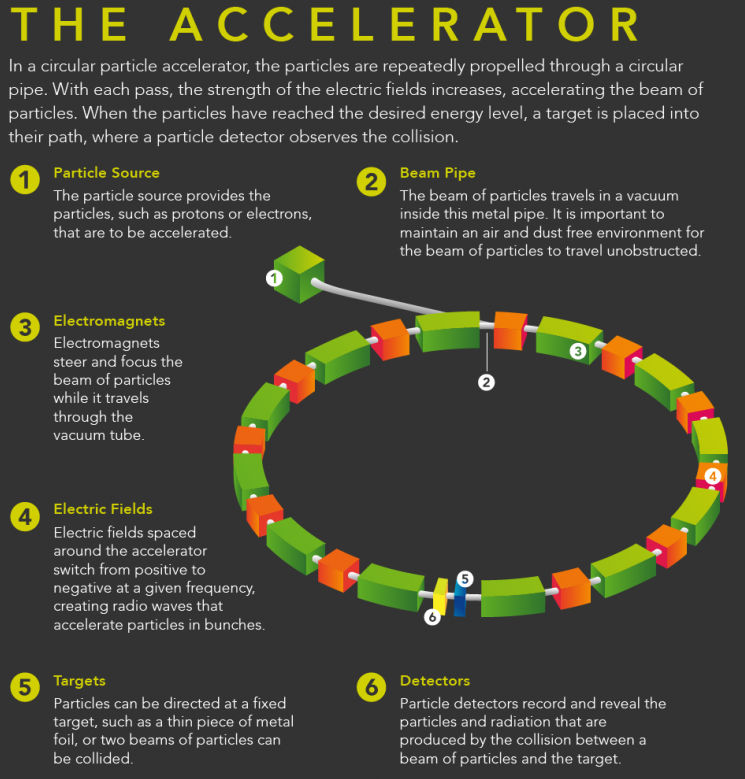
\includegraphics[width=0.9\textwidth]{fig/accelerators/0_CircularAccelerator}
\caption{A sketch of a circular accelerator with its basic components (from \href{http://energy.gov/articles/how-particle-accelerators-work}{http://energy.gov/articles/how-particle-accelerators-work}).
\label{fig:my_label}}
\end{figure}

\subsubsection{Circular versus linear}
There are two basic technologies: circular end linear accelerators. Circular accelerators have the advantage that one can give the accelerated particles a kick every time they come around, and also re-use those particles that did not disappear in the collision. They also allow a more compact design than linear accelerators. However, if one bends electrons or positrons around a circle (which is a type of acceleration) they loose a lot of energy through bremsstrahlung. This motivates the choice of linear accelerators for the next generation of very high energy electron-positron collider.

\subsubsection{Heavy particles for maximum energy}
The power $P$ of the bremsstrahlung emitted is proportional to $\gamma^4 = E^4/m^4$. For the same energy $E$, an electron looses $m_p^4/m_e^4 \approx 2000^4 = 16\cdot 10^{12}$ more energy than a proton. Therefore, protons can be accelerated to very high energies in a circular collider, without loosing significant amounts of energy through bremsstrahlung.
Proton colliders have therefore serious advantages for exploring the energy frontier (even though, as we shall see below, not all of the cm energy in proton collisions is available to produce new particles).

\subsubsection{Fixed target or collider? }
Once the particles have been accelerated, they need to be smashed into some target, or each other. In a fixed target experiment, the beam is dumped into some material. This is the technology of choice if the priority is to achieve high luminosities (high probability of some interaction is very high), and you don't care that you are colliding nuclei/protons (which are composite particles - see next section). The other option is collider experiment, where two beams are steered into each other. This is obviously much more challenging, and typically, only a few particles interact in each collision, so the luminosity is lower. But, as you learnt in the section on kinematics, far higher energies can be achieved this way, so if the purpose is to explore the energy frontier, you need to build a collider.

\subsubsection{Sledge-Hammer or scalpel?}
One of the most important differences between colliding protons with protons as in the LHC (or proton with antiproton as in the now decommissioned Tevatron), in contrast to electrons with positrons is due to the fact the electrons and positrons are fundamental particles, while protons are not.
\\\exercise{
Calculate the de-Broglie wavelength of a proton at the LHC in the cm system. How does this compare to the size of the proton?\vspace{2ex}\\
\rotatebox{180}{\parbox{0.95\textwidth}{$\lambda = \frac{h}{p}$ with $p=6.5TeV$ in the cm frame, and $h=2\pi \cdot 196\,\mathrm{MeV\,fm}$, $\lambda = 1.9\E{-4} \mathrm{fm}$, much smaller than the size of a proton of $\sim 1\mathrm{fm}$
}}}\\
At LHC energies (remember, high energies mean small distance scales), the proton is a complicated system of quarks and gluons. Each particle in this system is generically called a "parton". These partons are
\begin{itemize}
\item the valence quarks $uud$
\item gluons
\item sea quarks: quark-antiquark pairs that fleet in and out of existence. These are mainly light quarks $u\overline{u}$, $d\overline{d}$, and (less) $s\overline{s}$, but $c\overline{c}$ also plays a significant role.
\end{itemize}

\begin{figure}
\centering
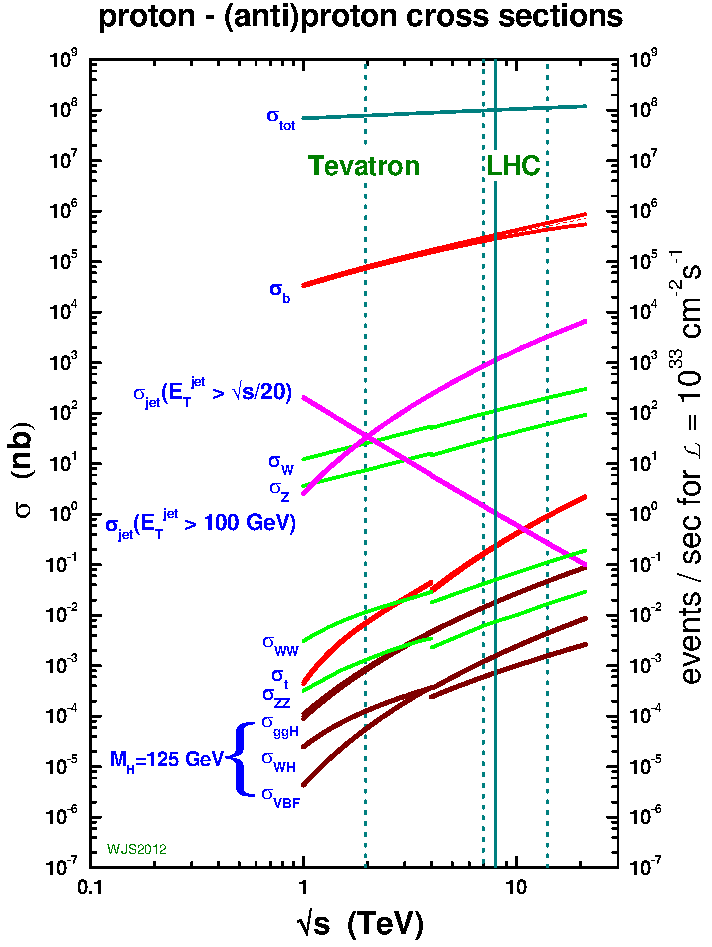
\includegraphics[width=0.7\textwidth]{fig/pp_xsection}
\caption{This plot shows the production cross section for $p\overline{p}$ (for $\sqrt{s}\le \un{4}{TeV}$) and $pp$ collisions (for $\sqrt{s} > \un{4}{TeV}$) as a function of the cm energy $\sqrt{s}$. Notice that the total $pp$ cross section is $10^{10}$ times bigger than that for Higgs production. The production cross section for $b\overline{b}$ is still $100,000,000$ time larger, meaning that the dominant Higgs decay mode $H \to b\overline{b}$ is completely drowned out by background. Note that one physicist's background is another physicist's signal: those huge numbers of $b\overline{b}$ events make LHCb the world-leading B-physics experiment.
From \href{inspirehep.net/record/810127?ln=en}{Eur.Phys.J. C63 (2009) 189-285} and \href{www.hep.ph.ic.ac.uk/~wstirlin/plots/plots.html}{www.hep.ph.ic.ac.uk/$\sim$wstirlin/plots/plots.html}.}
\end{figure}
At LHC energies the vast majority of the proton's energy is carried by gluons, so to first approximation, the LHC really is a gluon collider. The other big difference is of course that protons (and their constitutents) interact strongly, while electrons and positrons do not. Strong collisions tend to create far more particles in a collision.

\begin{figure}
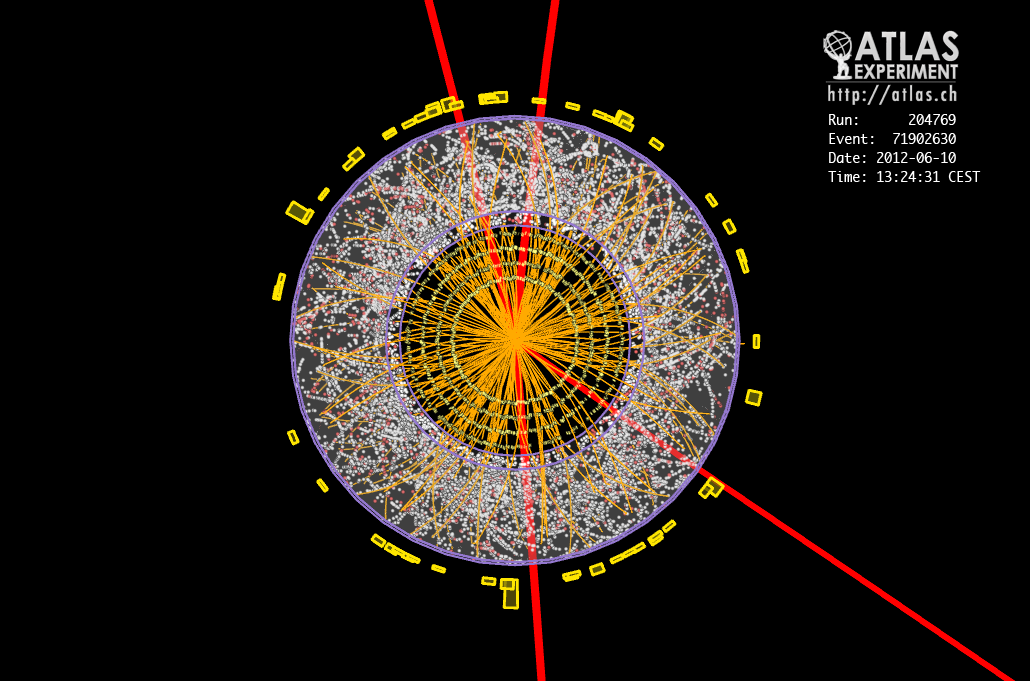
\includegraphics[width=0.58\textwidth]{fig/ATLAS_run204769_evt71902630}
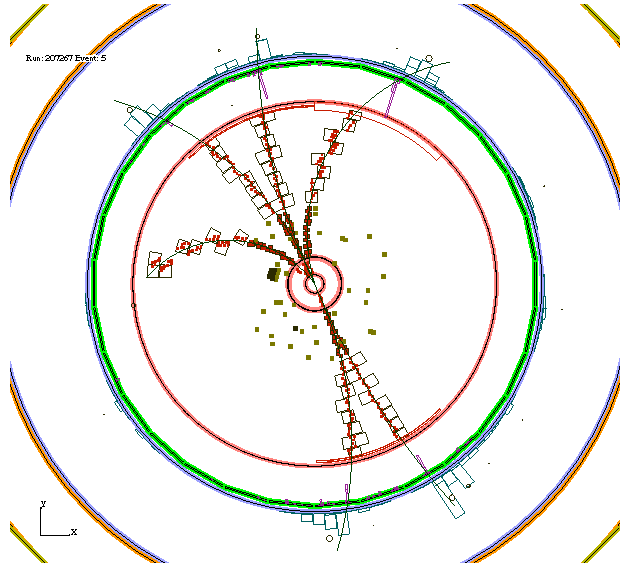
\includegraphics[width=0.4\textwidth]{fig/CLEOc_D2Kspipi_D2Kpi_Event}
\caption{Left: ATLAS event display for a p-p collision at the LHC. Two effects are compounded: The large number of track in each event, and the fact that that the LHC, multiple p-p collisions can happen in a single event. Right: CLEO-c event at an $e^+ e^-$ collider. Far fewer tracks are visible (in this case 6 tracks resulting from the process from $e^+ e^- \to \psi(3770) \to D\overline{D} \to (K_S\pi^+\pi^-)_D (K^+\pi^-)_{\overline{D}}$; the $K_S$ decayed to $\pi^+ \pi^-$) making reconstruction easier and cleaner.}
\end{figure}


The composite nature of the proton has the consequence that we do not know a priory what we are colliding. Most of the time, gluons, but with unknown momenta. 
This has the advantage that, at one proton collision energy, one can probe a wide range of gluon collision energies at the same time (good for discovery of unknown resonances/particles). 
It has the disadvantage that only some of the energy is available for the collision, and also that we do not know that energy, or the center of mass of the system. 

\subsubsection{Detecting invisible Particles}
\paragraph{Missing momentum in $e^+ e^-$ colliders}
\begin{figure}
\centering
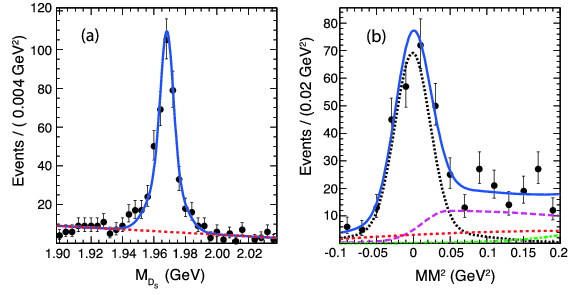
\includegraphics[width=0.9\textwidth]{fig/CLEO_Ds2munu}
\caption{Two plots from the reconstruction of \prt{D_s^+ \to \mu^+ \nu_{\mu}}: Left: the reconstructed mass-squared of the \prt{D_s} meson. Right: The reconstructed mass of the neutrino, inferred from the missing 4-momentum. The various lines show different contributions to the fit, with black-dotted signal, and the others different backgrounds (most prominently \prt{D_s^+ \to \tau^+ \nu_{\tau}} in pink-dashed). This clean reconstruction of invisible particles is only possible when the initial 4-momentum is known, as in an $e^+ e^-$ collider.
From: \href{https://inspirehep.net/record/810661/}{Phys.Rev. D79 (2009) 052001} \href{https://inspirehep.net/record/810661/}{[arXiv:0901.1216]}
\label{fig:CLEO_Ds2munu}}
\end{figure}

In electron-positron colliders, if one invisible particle (like a neutrino, or perhaps a dark matter particle) leaves the detector un-detected, we can still reconstruct its energy and momentum because we know the energies and momenta of the initial state and the other particles (see for example \figref{fig:CLEO_Ds2munu}. This is not possible at proton-proton collider. 

\paragraph{Missing transverse momentum (or $E_T$) in $p-p$ colliders}
\label{sec:missingEt}
\begin{figure}
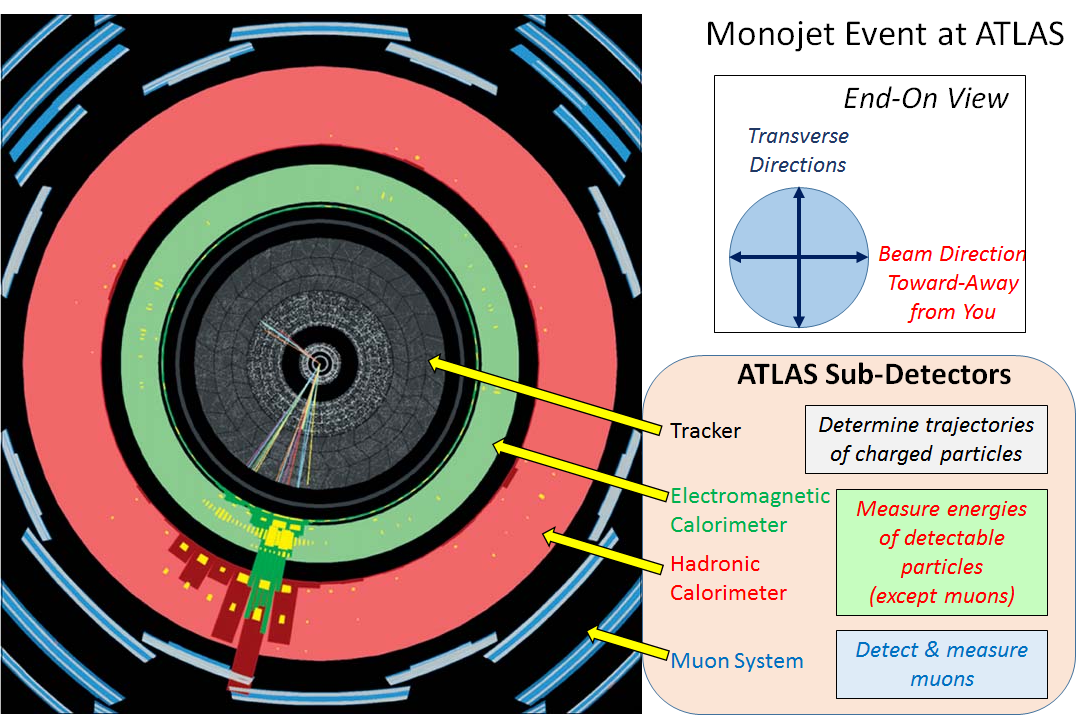
\includegraphics[width=0.52\textwidth]{fig/ATLAS_pp2nunuj_atlas}
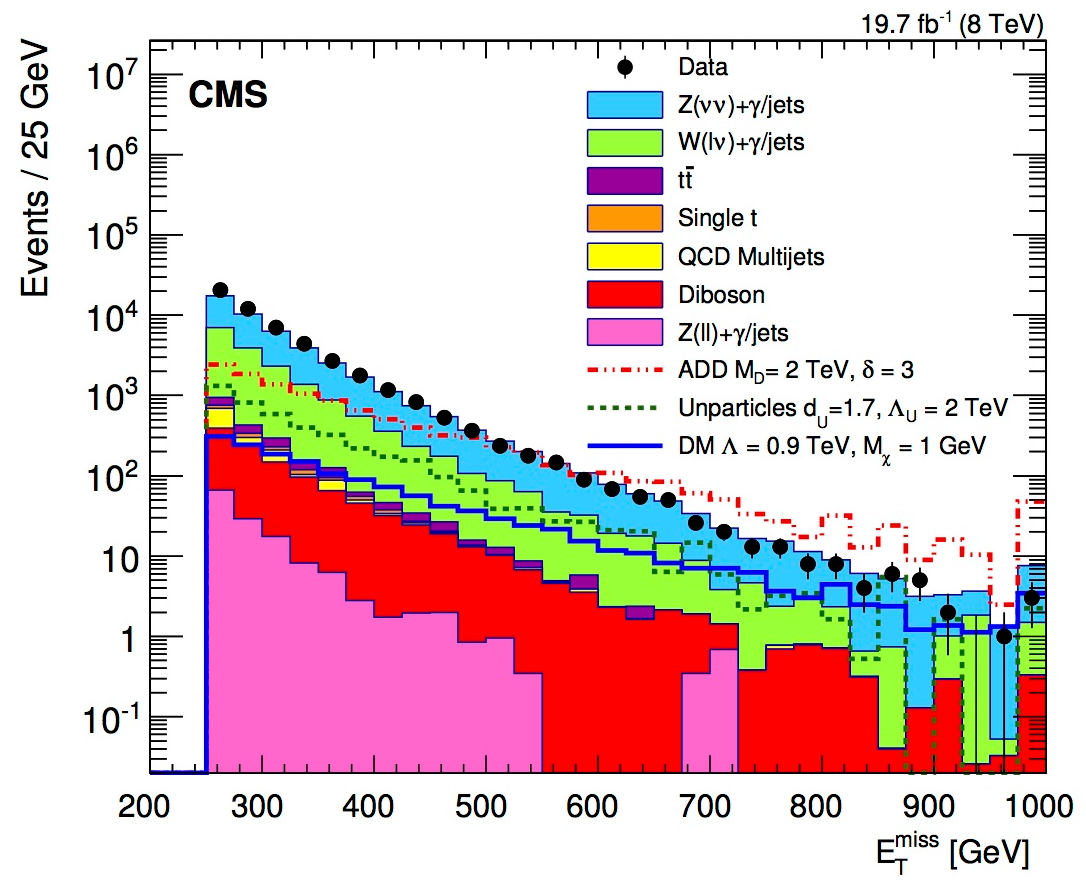
\includegraphics[width=0.45\textwidth]{fig/CMS_missingEtSpectrum}
\caption{Left: Event display from ATLAS (only showing high-energy tracks) with large missing $E_T$.
Right: Search for invisible heavy particles at CMS. The stacked coloured histograms correspond to missing $E_T$ signals from known standard model processes. The black dots represent the data. The dashed line corresponds to the signal expected in a certain New Physics model. Unfortunately, no new physics was seen, here.
\label{fig:missingET_atLHC}
}
\end{figure}

However, we can still do something even at proton-proton colliders: we know that the cm system has no transverse momentum, so the momenta perpendicular to the beam line mucht add up to zero. Often this is called transverse energy, $E_T$ but what is really meant by this is the magnitude of the \emph{vector} sum the momenta transverse to the beam direction:
\begin{equation}
E_T = \left|
\sum\limits_{\mathrm{i=all\;particles\;in\;collision}} \vec{p}_{Ti} \right|
\end{equation}
where $\vec{p}_{Ti} = (p_{ix}, p_{iy}, 0)$ is the transverse momentum of the $i$th particle and $z$ is the direction along the beam line. This needs to add up to zero if all particles have been detected. If it doesn't, we know that some particle has escaped undetected.

The complicated structure of the colliding protons, and the fact that they are made from strongly interacting particles, also results in the creation of a lot of particle jets in addition to creation and decay of the particles of interest (like the Higgs). 
The Higgs discovery is actually a nice example to illustrate the challenges (as well as the success) of the doing particle physics at hadron colliders: 
It is for these challenges, that the Higgs was not detected in its dominant decay mode, \prt{H \to b\overline{b}}. In the strong interaction processes at the LHC's proton-proton collisions, lots of $b\overline{b}$ quark pairs are produced, so the background to \prt{H \to b\overline{b}} is overwhelming. 
(BTW, the LHCb experiment uses this exact feature as its advantage and studies these huge quantities of $b\overline{b}$ quarks, and the mesons and baryons they form, for high precision flavour physics (i.g. \cpv) measurements.) 
The next heaviest pair of particles the Higgs can decay to is $\tau^+\tau^-$. But that is also really difficult to reconstruct, because the decay of each $\tau$ involves at least one neutrino (difficult, because we have no way to fully reconstruct its energy/momentum) and a virtual $W$. That $W$ can then either decay to leptons (which means more neutrinos, i.e. missing energy) or to jets (lots of background from QCD processes). 
At the end, the main discovery channels for the $H$ were \prt{H \to \gamma \gamma} (which proceeds via a loop diagram) and \prt{H \to 4\ell} ($\ell$ stands for $e^+$ or $e^-$ or $\mu^+$ or $\mu^-$) via an intermediate state of two $Z$ bosons (one virtual, one 'real'). 
Both of these are fairly rare, but "easy" to see, because they don't involve invisible particles, and they don't involve hadrons (strongly interacting particles) in the final state, and thus there is less background from all the QCD processes that go on in a hadron collider.

\subsubsection{Summary: $e^+ e^-$ vs $pp$}
The advantage of an electron-positron collider is then that the initial state is very well known, and the interaction is "clean", i.e. has less background. And if one knows where to look, one can tune the collider to the appropriate cm energy. It's ideal for precision studies. 
Therefore people are proposing to build a $e^+\,e^-$ collider (either circular or linear) to study the Higgs, and possibly (if the LHC finds any evidence for it), new particles beyond the SM. 
While for studying the Higgs, it is unclear if a linear or a circular collider is better, studying heavy new particles with masses in the TeV range would require a linear collider - circular ones would loose too much energy through bremsstrahlung to reach this energy. On the other hand, if we wanted to search for new heavy particles beyond the energies currently reached by the LHC, the best choice for achieving such high high energies is a proton-proton collider.

\exercise{In what way would a muon collider be the "ideal" collider? Why haven't we built one?}
